
\newcommand{\TikzPtheta}[2]{
\draw[#1] (4.5, 3)  node[anchor=north] {#2};
\begin{scope}[shift={(2.5,2.5)}]
    \begin{scope}[rotate=45]
        \begin{scope}[shift={(-2.5,-2.5)}]
            \foreach \s in {0.2, 0.4, 0.6, 0.8, 1.0}
            \draw[#1] (2.5,2.5) ellipse (\s * 3 and \s * 1);
        \end{scope}
    \end{scope}
\end{scope}
}


\newcommand{\TikzPlotArea}{
\draw (0,0)--(5,0);
\foreach \x in {0,...,5}
  \draw (\x,0)--(\x,-.1) node[anchor=north]{};

\draw (0,0)--(0,5);
\foreach \y in {0,...,5}
  \draw (0,\y)--(-.1,\y) node[anchor=east] {};

\draw (0,5) node[anchor=east] {$\theta_2$};
\draw (5,0) node[anchor=north] {$\theta_1$};
}


%%%%%%%%%%%%%%%%%%%%%%%%%%%%%%%%%%%%%%%%%%%%%%%%%%%%%%%%%%%%%%%%%%%%%%%%%%%%%%
%%%%%%%%%%%%%%%%%%%%%%%%%%%%%%%%%%%%%%%%%%%%%%%%%%%%%%%%%%%%%%%%%%%%%%%%%%%%%%
%%%%%%%%%%%%%%%%%%%%%%%%%%%%%%%%%%%%%%%%%%%%%%%%%%%%%%%%%%%%%%%%%%%%%%%%%%%%%%

\begin{frame}{KL divergence exercises}
\begin{minipage}{0.5\textwidth}
%
\begin{align*}
%
\p(\theta) ={}& \textrm{Correlated bivariate normal}\\ \\
%
\qdom ={}& \left\{ \textrm{All bivariate normals}\right\}\\ \\
%
\end{align*}
%
What is
$\qopt(\theta) = \argmin{\q \in \qdom} \kl{\q(\theta)}{\p(\theta)}$?
%
\end{minipage}
%
\begin{minipage}{0.4\textwidth}

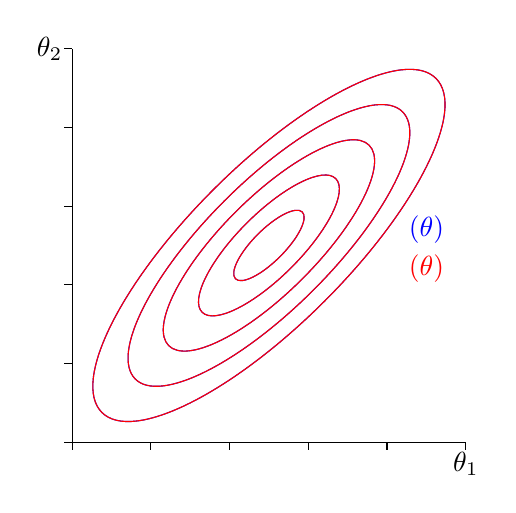
\begin{tikzpicture}
\TikzPlotArea{}
\TikzPtheta{blue}{$\p(\theta)$}

\onslide<2->{
\TikzPtheta{red}{}
\draw[red] (4.5, 2.5)  node[anchor=north] {$\qopt(\theta)$};
}
\end{tikzpicture}
\end{minipage}

\end{frame}


%%%%%%%%%%%%%%%%%%%%%%%%%%%%%%%%%%%%%%%%%%%%%%%%%%%%%%%%%%%%%%%%%%%%%%%%%%%%%%
%%%%%%%%%%%%%%%%%%%%%%%%%%%%%%%%%%%%%%%%%%%%%%%%%%%%%%%%%%%%%%%%%%%%%%%%%%%%%%
%%%%%%%%%%%%%%%%%%%%%%%%%%%%%%%%%%%%%%%%%%%%%%%%%%%%%%%%%%%%%%%%%%%%%%%%%%%%%%

\begin{frame}{KL divergence exercises}
\begin{minipage}{0.5\textwidth}
    %
\begin{align*}
%
\p(\theta) ={}& \textrm{Correlated bivariate normal}\\ \\
%
\qdom ={}& \left\{ \textrm{Independent bivariate normals}\right\}\\ \\
%
\end{align*}
%
What is
$\qopt(\theta) = \argmin{\q \in \qdom} \kl{\q(\theta)}{\p(\theta)}$?
%
\end{minipage}
%
\begin{minipage}{0.4\textwidth}

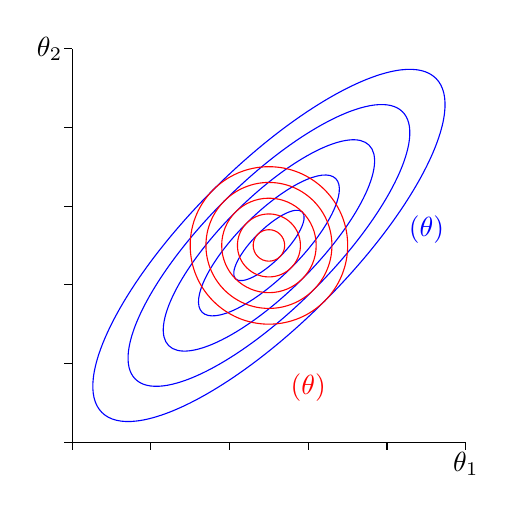
\begin{tikzpicture}
\TikzPlotArea{}
\TikzPtheta{blue}{$\p(\theta)$}

\onslide<2->{
\draw[red] (3, 1)  node[anchor=north] {$\qopt(\theta)$};
\foreach \s in {0.2, 0.4, 0.6, 0.8, 1.0}
    \draw[red] (2.5,2.5) ellipse (\s * 1 and \s * 1);
}
\end{tikzpicture}
\end{minipage}

\end{frame}




%%%%%%%%%%%%%%%%%%%%%%%%%%%%%%%%%%%%%%%%%%%%%%%%%%%%%%%%%%%%%%%%%%%%%%%%%%%%%%
%%%%%%%%%%%%%%%%%%%%%%%%%%%%%%%%%%%%%%%%%%%%%%%%%%%%%%%%%%%%%%%%%%%%%%%%%%%%%%
%%%%%%%%%%%%%%%%%%%%%%%%%%%%%%%%%%%%%%%%%%%%%%%%%%%%%%%%%%%%%%%%%%%%%%%%%%%%%%

\begin{frame}{KL divergence exercises}
\begin{minipage}{0.5\textwidth}
    %
\begin{align*}
%
\p(\theta) ={}& \textrm{Correlated bivariate normal}\\ \\
%
\qdom ={}& \left\{ \textrm{Independent bivariate normals}\right\}\\ \\
%
\end{align*}
%
What is
$\qopt(\theta) ={} \argmin{\q \in \qdom} \kl{\p(\theta)}{\q(\theta)}$?
%
\end{minipage}
%
\begin{minipage}{0.4\textwidth}

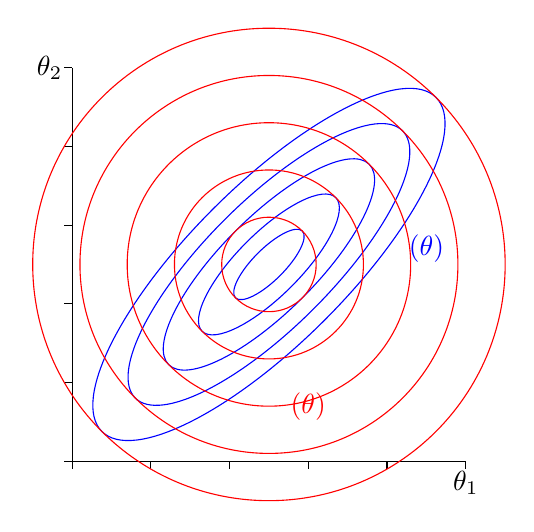
\begin{tikzpicture}
\TikzPlotArea{}
\TikzPtheta{blue}{$\p(\theta)$}

\onslide<2->{
\draw[red] (3, 1)  node[anchor=north] {$\qopt(\theta)$};
\foreach \s in {0.2, 0.4, 0.6, 0.8, 1.0}
    \draw[red] (2.5,2.5) ellipse (\s * 3 and \s * 3);
}
\end{tikzpicture}
\end{minipage}

\end{frame}




%%%%%%%%%%%%%%%%%%%%%%%%%%%%%%%%%%%%%%%%%%%%%%%%%%%%%%%%%%%%%%%%%%%%%%%%%%%%%%
%%%%%%%%%%%%%%%%%%%%%%%%%%%%%%%%%%%%%%%%%%%%%%%%%%%%%%%%%%%%%%%%%%%%%%%%%%%%%%
%%%%%%%%%%%%%%%%%%%%%%%%%%%%%%%%%%%%%%%%%%%%%%%%%%%%%%%%%%%%%%%%%%%%%%%%%%%%%%

\begin{frame}{KL divergence exercises}
\hspace{-3em}
\begin{minipage}{0.5\textwidth}
%
Recall that
\begin{align*}
%
\MoveEqLeft
\kl{\q(\theta)}{\p(\theta)} ={}\\&
-\expect{\q(\theta)}{\log \p(\theta)} +
\expect{\q(\theta)}{\log \q(\theta)}\\ \\
\p(\theta) ={}& \textrm{Correlated bivariate normal}\\ \\
\qdom ={}& \left\{ \textrm{Bivariate normals}\right\}
%
\end{align*}

What is $\qopt(\theta) = $\\
$\argmin{\q \in \qdom}
\Big(-\expect{\q(\theta)}{\log \p(\theta)} +$
\sout{$\expect{\q(\theta)}{\log \q(\theta)} \Big)$}?
%
\end{minipage}
%
\begin{minipage}{0.4\textwidth}

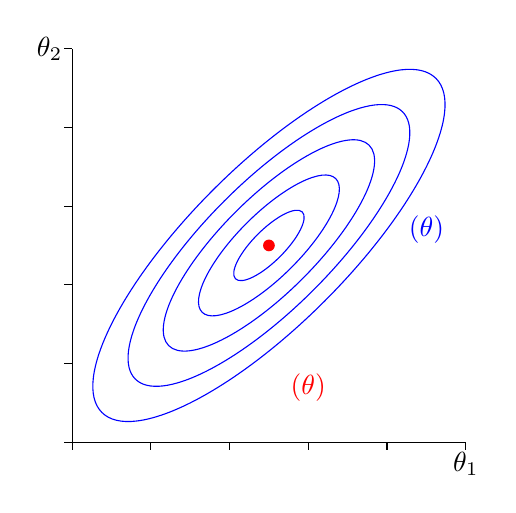
\begin{tikzpicture}
\TikzPlotArea{}
\TikzPtheta{blue}{$\p(\theta)$}

\onslide<2->{
\draw[red] (3, 1)  node[anchor=north] {$\qopt(\theta)$};
\node at (2.5,2.5) [circle,fill=red,inner sep=1.5pt]{};
}
\end{tikzpicture}
\end{minipage}

\end{frame}



%%%%%%%%%%%%%%%%%%%%%%%%%%%%%%%%%%%%%%%%%%%%%%%%%%%%%%%%%%%%%%%%%%%%%%%%%%%%%%
%%%%%%%%%%%%%%%%%%%%%%%%%%%%%%%%%%%%%%%%%%%%%%%%%%%%%%%%%%%%%%%%%%%%%%%%%%%%%%
%%%%%%%%%%%%%%%%%%%%%%%%%%%%%%%%%%%%%%%%%%%%%%%%%%%%%%%%%%%%%%%%%%%%%%%%%%%%%%

\begin{frame}{KL divergence exercises}
\hspace{-3em}
\begin{minipage}{0.5\textwidth}
%
Recall that
\begin{align*}
%
\MoveEqLeft
\kl{\q(\theta)}{\p(\theta)} ={}\\&
-\expect{\q(\theta)}{\log \p(\theta)} +
\expect{\q(\theta)}{\log \q(\theta)}\\ \\
\p(\theta) ={}& \textrm{Correlated bivariate normal}\\ \\
\qdom ={}& \left\{ \textrm{Bivariate normals}\right\}
%
\end{align*}

What is $\qopt(\theta) = $\\
$\argmin{\q \in \qdom} \Big(-$
\sout{$\expect{\q(\theta)}{\log \p(\theta)}$}
$+ \expect{\q(\theta)}{\log \q(\theta)} \Big)$?
%
\end{minipage}
%
\begin{minipage}{0.4\textwidth}

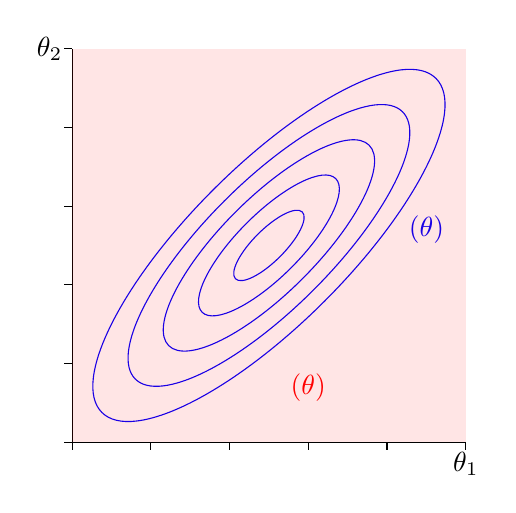
\begin{tikzpicture}
\TikzPlotArea{}
\TikzPtheta{blue}{$\p(\theta)$}

\onslide<2->{
\draw[red] (3, 1)  node[anchor=north] {$\qopt(\theta)$};
%\node at (2.5,2.5) [circle,fill=red,inner sep=1.5pt]{};
\draw[draw opacity=0, fill opacity=0.1, fill=red] (0,0) rectangle (5, 5);

}
\end{tikzpicture}
\end{minipage}

\end{frame}
